
\begin{exercice}[Partiel 2017-18]
On utilise la structure de donnée suivante :

\begin{lstlisting}
Structure Cellule:
    Entier valeur
    Cellule suivante

Structure Liste:
    Cellule premiere
\end{lstlisting}

Donner un algorithme qui prend en entrée une liste chaînée dont on suppose les valeurs ordonnées et qui supprime les occurrences multiples.

Par exemple, si la liste est 
\scalebox{.8}{
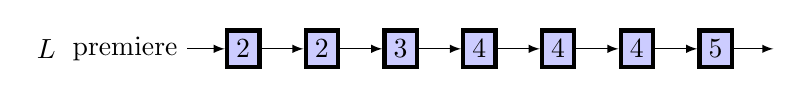
\begin{tikzpicture}[>=latex]
\node(L) at (-2,0){$L$};
\node(Prem) at (-1,0){premiere};

\node(T1)[draw, ultra thick, fill=blue!20, rectangle] at (0.5,0) {2};
\node(T2)[draw, ultra thick, fill=blue!20, rectangle] at (1.5,0) {2};
\node(T3)[draw, ultra thick, fill=blue!20, rectangle] at (2.5,0) {3};
\node(T4)[draw, ultra thick, fill=blue!20, rectangle] at (3.5,0) {4};
\node(T5)[draw, ultra thick, fill=blue!20, rectangle] at (4.5,0) {4};
\node(T6)[draw, ultra thick, fill=blue!20, rectangle] at (5.5,0) {4};
\node(T7)[draw, ultra thick, fill=blue!20, rectangle] at (6.5,0) {5};

\draw (Prem.east) edge[->] (T1.west);
\draw (T1.east) edge[->] (T2.west);
\draw (T2.east) edge[->] (T3.west);
\draw (T3.east) edge[->] (T4.west);
\draw (T4.east) edge[->] (T5.west);
\draw (T5.east) edge[->] (T6.west);
\draw (T6.east) edge[->] (T7.west);
\draw (T7.east) edge[->] ++(.5,0);
\end{tikzpicture}
}

Le résultat après le passage de l'algorithme sera
\scalebox{.8}{
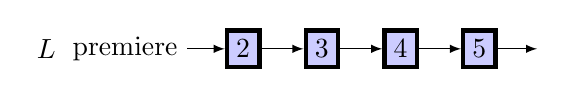
\begin{tikzpicture}[>=latex]
\node(L) at (-2,0){$L$};
\node(Prem) at (-1,0){premiere};

\node(T1)[draw, ultra thick, fill=blue!20, rectangle] at (0.5,0) {2};
\node(T2)[draw, ultra thick, fill=blue!20, rectangle] at (1.5,0) {3};
\node(T3)[draw, ultra thick, fill=blue!20, rectangle] at (2.5,0) {4};
\node(T4)[draw, ultra thick, fill=blue!20, rectangle] at (3.5,0) {5};

\draw (Prem.east) edge[->] (T1.west);
\draw (T1.east) edge[->] (T2.west);
\draw (T2.east) edge[->] (T3.west);
\draw (T3.east) edge[->] (T4.west);
\draw (T4.east) edge[->] ++(.5,0);
\end{tikzpicture}
}

\vspace{0.5cm}

\textbf{Solution}

Un algorithme possible (ce n'est pas le seul)

\begin{lstlisting}
Input : Une liste L
Procédé :
	c <- L.premiere
	Si c != None:
	   Tant que c.suivante != None:
	       v <- c.valeur
	       Si c.suivante.valeur == v:
	           c.suivante <- c.suivante.suivante
	       Sinon :
	           c <- c.suivante
\end{lstlisting}

Question donnée au partiel 1 2017-2018, résultats obtenus :

\begin{tabular}{|c|c|c|c|c|}
\hline
A & B & C & D & E \\ \hline
$28.6\%$ & $19\%$ & $42.9\%$ & $9.5\%$ & $0\%$ \\ \hline
\end{tabular} 

\vspace{0.5cm}

Exemple d'un algorithme qui obtient "B" :

\begin{lstlisting}
c <- L.premiere
Tant que c.suivante != None:
   v <- c.valeur
   Si c.suivante.valeur == v:
       c.suivante <- c.suivante.suivante
   Sinon :
       c <- c.suivante
\end{lstlisting}

Oubli de tester si \texttt{L.premiere} est \texttt{None} avant de faire \texttt{c.suivante} : l'algo ne fonctionne pas sur la liste vide.

Exemple d'un algorithme qui obtient "C" (le plus courant)

\begin{lstlisting}
c <- L.premiere
Si c != None:
   Tant que c.suivante != None:
       v <- c.valeur
       Si c.suivante.valeur == v:
           c.suivante <- c.suivante.suivante
       c <- c.suivante
\end{lstlisting}

On passe systématiquement à \texttt{c.suivante} : cet algorithme ne fonctionne pas dès qu'il y a plus de 2 copies d'une même cellule.

\end{exercice}